


\label{sec:evaluation}

This section answers the following questions:
\begin{itemize}
\item
  How effective is \Predator{} at detecting and predicting false sharing?

\item
  What is \Predator{}'s overhead, in terms of execution time and memory ?

\item
  How sensitive is \Predator{} to different sampling rates?
 
\end{itemize}

\paragraph{Experimental Platform.} All evaluations are performed on a quiescent Intel Core 2 dual-processor system,  equipped with 16GB RAM in total. Each processor is a 4-core 64-bit Intel Xeon running at 2.33 GHz, with a 4MB shared L2 cache and 32KB private L1 cache. The underlying operating system is an unmodified CentOS 5.5, running with Linux kernel version 2.6.18-194.17.1.el5. The glibc version is 2.5. 

\paragraph{Evaluated Applications.}
This paper evaluates two popular benchmark suites,
Phoenix (with large input) ~\cite{phoenix-hpca} and PARSEC (with simlarge input) ~\cite{parsec}. Even with unmodified LLVM-3.2, Facesim cannot be compiled successfully (having complaints on an undefined template) and Canneal aborts unexpectedly. Thus, these two benchmarks are excluded.
We also evaluate \Predator{} on six real applications, including MySQL, Boost, Memcached, aget, pbzip2 and pfscan.



\subsection{Detection and Prediction Effectiveness}
\label{sec:predatoreffective}

\begin{figure*}[htb]
{\centering
\tiny
\subfigure{\lstinputlisting[numbers=none,frame=none,boxpos=t]{predator/figure/linearregression.report}}
\caption{An example reported by \Predator{}, indicating a potential false sharing problem in the linear\_regression benchmark.
\label{fig:lrreport}}
}
\end{figure*}

For every false sharing problem, \Predator{} reports source code information and detailed memory access information in order to help users fix those problems. Figure~\ref{fig:lrreport} shows an example for the linear\_regression benchmark. This report shows that the heap object starting with $0x40000038$ potentially causes a large number of cache invalidations. The call stack of this memory allocation is provided to help locate culprits. In addition, \Predator{} also reports word-level access information of this object, which helps to identify where and how false sharing occurs. From that, we can know that it is a latent false sharing problem predicted by \Predator{}, since different threads are accessing different cache lines. 

\subsubsection{Benchmarks}
\label{sec:benchmarks}

\begin{table}[!t]
{\centering
\resizebox{\columnwidth}{!}{
\begin{tabular}{l|r|r|r|r|r}\hline
{\bf \small Benchmark} & {\bf \small Source Code} & {\bf \small New} & {\bf \small Without Prediction} &{\bf \small With Prediction} & {\bf \small Improvement} \\
\hline
\small \textbf{histogram} & {\small histogram-pthread.c:213} & \cmark{} &\cmark{} & \cmark{} & 46.22\%\\
\small \textbf{linear\_regression} & {\small linear\_regression-pthread.c:133} & & & \cmark{} & 1206.93\% \\
\small \textbf{reverse\_index} & {\small reverseindex-pthread.c:511} & & \cmark{} & \cmark{} & 0.09\%\\
\small \textbf{word\_count} & {\small word\_count-pthread.c:136} & & \cmark{} & \cmark{} & 0.14\%\\
\hline
\small \textbf{streamcluster} & {\small streamcluster.cpp:985} &  & \cmark{} & \cmark{} &7.52\% \\
\small \textbf{streamcluster} & {\small streamcluster.cpp:1907} & \cmark{} & \cmark{} & \cmark{} & 4.77\%\\
\hline
\end{tabular} }
\caption{False sharing problems in the Phoenix and PARSEC benchmark suites. \label{table:detection}}
}
\end{table}

We evaluate \Predator{}'s effectiveness on two benchmark suites, Phoenix and PARSEC, and Table~\ref{table:detection} presents those benchmarks with false sharing problems. 
The first column lists those programs with false sharing problems.  The second column shows precisely where the problem is. Because all discovered false sharing occurs inside heap objects, we show the source code information of callsite here.  The third column, ``New'', marks whether this false sharing was newly discovered by \Predator{}.  A checkmark in the  following two columns indicates whether the false sharing was identified without prediction or with prediction enabled.  The final column, ``Improvement'', shows the performance improvement after fixing false sharing. Note that the performance improvement shown here is different with that in Table~\ref{table:perfafterfix} because \SheriffDetect{} evaluates on a 32bit platform and \Predator{} evaluates on a 64bit platform. This also shows that performance effect is every sensitive to hardware platform, which is one of dynamic properties that we discussed above. 
%The number is based on the average runtime of $10$ runs. 

As shown in the table, \Predator{} reveals two unknown false sharing problems. It is the first tool to uncover false sharing in histogram and at line $1907$ of streamcluster. 
In histogram, multiple threads simultaneously modify different locations of the same heap object, thread\_arg\_t. 
Padding this data structure fixes the false sharing problem and improves the performance by around 46\%. In streamcluster, multiple threads are simultaneously accessing and updating the same \texttt{bool} array, switch\_membership. Simply changing all elements of this array to a long type reduces the false sharing effect, improving performance by about 4.7\%.

%, although it is not a complete fix of false sharing. 
%None of these two false sharing problems has been reported by previous tools.
Other false sharing problems were discovered by previous work~\cite{sheriff}. The detailed reason of false sharing problems and how they are fixed are discussed in Section~\ref{sec:effecteval}.

It is worth noting that linear\_regression has a potential false sharing problem according to the execution environment of \Predator{}. According to the observation of Nanavati et al., this false sharing problem occurs when using clang and disappears when using gcc with the -O2 and -O3 optimization level~\cite{OSdetection}. But we observed a different result: when we are using the clang-3.2 compiler and our custom memory allocator, the false sharing problem does not occur at all because the offset happens to be 56 bytes (see Figure~\ref{fig:perfsensitive}). 
However, it does occur in the original execution environment, with the default memory allocator and using gcc compiler. That is why fixing it improves the performance by more than $12\times$.  This also exemplifies the necessity of \Predator{} predictive detection: existing tools may miss a false sharing problem if it does not occur at their test environments. 
 
\subsubsection{Real Applications}
To verify \Predator{}'s practicality, we further evaluate several widely-used real applications, whereas no previous work has done this. These real applications include a server application (MySQL~\cite{mysql}),
a standard C++ library (Boost~\cite{libfalsesharing}),
a distributed memory object caching system (Memcached), a network retriever (aget),
a parallel bzip2 file compressor (pbzip2), and a parallel file scanner (pfscan).

MySQL-5.5.32 and boost-1.49.0 are known to have false sharing problems. Other applications (memcached-1.4.15, aget-0.4.1,  pbzip2-1.1.6, and pfscan) do not have known false sharing problems.

The false sharing of MySQL has caused a significant scalability problem and was very difficult to be identified.
According to the architect of MySQL, Mikael Ronstrom, ``we had gathered specialists on InnoDB..., participants from MySQL support... and a number of generic specialists on 
computer performance...'', ``[we] were able to improve MySQL performance by 6$\times$ with those scalability fixes''~\cite{mysql}. 
The false sharing inside Boost is caused by the usage of a  spinlock pool. Different threads may utilize different spinlocks located in the same cache line in this case. Reducing the number of spinlocks on per cache line to 1 brings a 40\% performance improvement.
\Predator{} is able to pinpoint false sharing locations in both MySQL and the Boost library. 
For the other four applications, \Predator{} does not find severe false sharing problems.

\subsubsection{Prediction Effectiveness}
\label{sec:predicteval}
In this section, we verify whether prediction can always  reveal un-observed false sharing problems.

The linear\_regression benchmark is evaluated here because of the following two reasons: (1) The false sharing problem of this benchmark cannot be detected without prediction; (2) The false sharing problem severely degrades performance when it actually occurs, thus it is a serious problem that should be detected. 

\begin{figure}
\begin{lstlisting} [style=tt]
struct
{
  pthread_t tid;  POINT_T *points;
  int num_elems;  long long SX;
  long long SY;   long long SXX;
  long long SYY;  long long SXY;
} lreg_args;

void * lreg_thread ( void * args_in ) {
  struct lreg_args * args = args_in ;
  for(i=0; i<args->num_elems; i++) {
    args->SX+=args->points[i].x;
    args->SXX+=args->points[i].x*args->points[i].x;
    args->SY+=args->points[i].y;
    args->SYY+=args->points[i].y*args->points[i].y;
    args->SXY+=args->points[i].x*args->points[i].y;
  }
}
\end{lstlisting}
\caption{The false sharing problem inside the linear\_regression benchmark: multiple threads simultaneously update distinct entries of a global array.
\label{fig:linearregression}}
\end{figure}

Figure~\ref{fig:linearregression} shows the data structure and the code exercising corresponding false sharing. The size of this data structure, lreg\_args, is $64$ bytes 
when the program is compiled to a $64$-bit binary using llvm compiler, with optimization level ``-O3''. In this benchmark, the main thread allocates an array, containing as the same number of elements as hardware cores. Each element is a lreg\_args type with $64$ bytes. This array is then passed to different threads (lreg\_thread function) so that each thread only updates its thread-dependent area. False sharing occurs if two threads happen to update a cache line. 

Figure~\ref{fig:perfsensitive} shows how sensitive the performance is to different starting addresses of this falsely-shared object. When the offset is $0$ or $56$ bytes, this benchmark achieves its optimal performance and has no false sharing. When the offset is $24$ bytes, the benchmark runs about $15$ times slower than its optimal performance because of the false sharing problem.

Our evaluation shows that \Predator{} can always detect the false sharing problem with prediction enabled, when this false  sharing object starts with different offsets. This demonstrates the effectiveness of its prediction mechanism.

\subsection{Performance Overhead}
\label{sec:perfoverhead}

\begin{figure*}[!t]
\centering
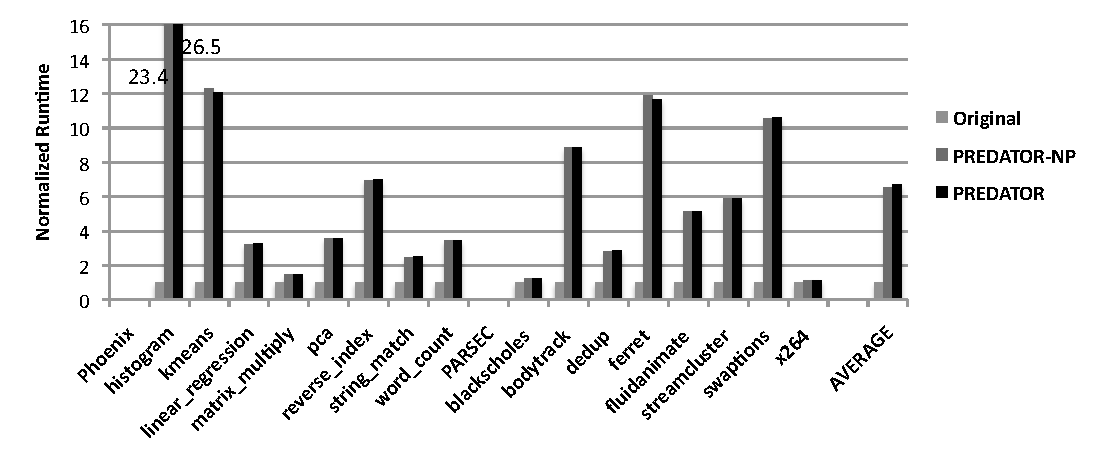
\includegraphics[width=6in]{predator/figure/perf}
\caption{
Performance overhead of \Predator{} with and without prediction(PREDATOR-NP).
\label{fig:perf}}
\end{figure*}
We perform evaluations on different benchmarks and application $10$ times and show the average of $8$ runs in in Figure~\ref{fig:perf}. To avoid the effect caused by extreme outliers, the maximum and minimum values are excluded here. 

For $16$ benchmarks from the Phoenix and PARSEC benchmark suites and six real applications, \Predator{} imposes $5.4\times$ performance overhead averagely. There is no noticeable difference on performance whether the prediction mechanism is enabled or not. 
 
Among five of these programs, histogram, kmeans, bodytrack, ferret, and swaptions, \predator{} introduces more than $8\times$ performance overhead. The histogram benchmark runs more than $26\times$ slower than the one with \pthreads{}, because tracking detailed access on cache lines with false sharing exacerbates the false sharing effect (see more discussion in Section~\ref{sec:sample}).  For bodytrack and ferret, although there is no false sharing, \Predator{} detects a large amount of cache lines with writes larger than {\it Tracking-Threshold}. Thus, tracking those accessing details for those cache lines imposes significant performance overhead. Currently, we have not identified the exact cause of \Predator{}'s high performance for kmeans.
   
\Predator{} imposes a small performance overhead for IO-bound applications, such as matrix\_multiply, blackscholes, x264, aget, Memcached, pbzip2, and pfscan, since \Predator{} does not add any performance overhead for IO operations.  

\subsection{Memory Overhead}
\label{sec:memoverhead}
We evaluate physical memory overhead of \Predator{}, instead of virtual memory overhead, because \Predator{} allocates 4GB virtual memory for its custom memory allocator beforehand. Proportional set size (PSS) of a specific memory mapping (in \texttt{/proc/self/smaps}) reflects the physical memory increase because of running the current application~\cite{memusage}. Thus, we periodically collect this data and use the sum of different memory mappings as the total physical memory usage of running an application. Figure~\ref{fig:memusage} presents the normalized physical memory usage of running different applications, comparing to that using \pthreads{}. 

\Predator{} imposes less than 50\% memory overhead for 17 out of 22 applications.  For swaptions and aget, \Predator{} introduces more memory overhead because the original memory footprints of them are very small, only $3$ kilobytes. Adding the code of detection, prediction and reporting (constant overhead) contributes to a large ratio of memory overhead. The increase of memory consumption in MySQL, from 132 MB to 512 MB, is due to \Predator{}'s heap organization, which does not aggressively reclaim memory held by individual threads. In all cases where \Predator{}'s imposes substantial memory overhead, the applications continue to comfortably fit into RAM on modern platforms.


\subsection{Sampling Rate Sensitivity}
\label{sec:predatorsensitivity}
Section~\ref{sec:sample} describes \Predator{}'s sampling mechanism to reduce tracking overhead. This section evaluates the effect of different sampling rates on performance and effectiveness. Note that running an application with different sampling rates does not affect its memory usage, thus memory overhead is not examined here. 

The default sampling rate used by \Predator{} is 1\%. In this section, we also evaluate two other sampling rates, 0.1\% and 10\%. Figure~\ref{fig:predatorsample} presents performance results under the three different sample rates. We only show the results of those programs having false sharing problems inside, since only their performance are most likely to be affected by different sampling rates. As expected, \Predator{} introduces less performance overhead under a lower sampling rate, but with a very minor performance impact. About effectiveness, even when using the 0.1\% sampling rate, \Predator{} can still detect all false sharing problems, although it reports a lower number of cache invalidations. Thus, different sampling rates do not affect the detection effectiveness.
 
\begin{figure*}[!t]
\centering
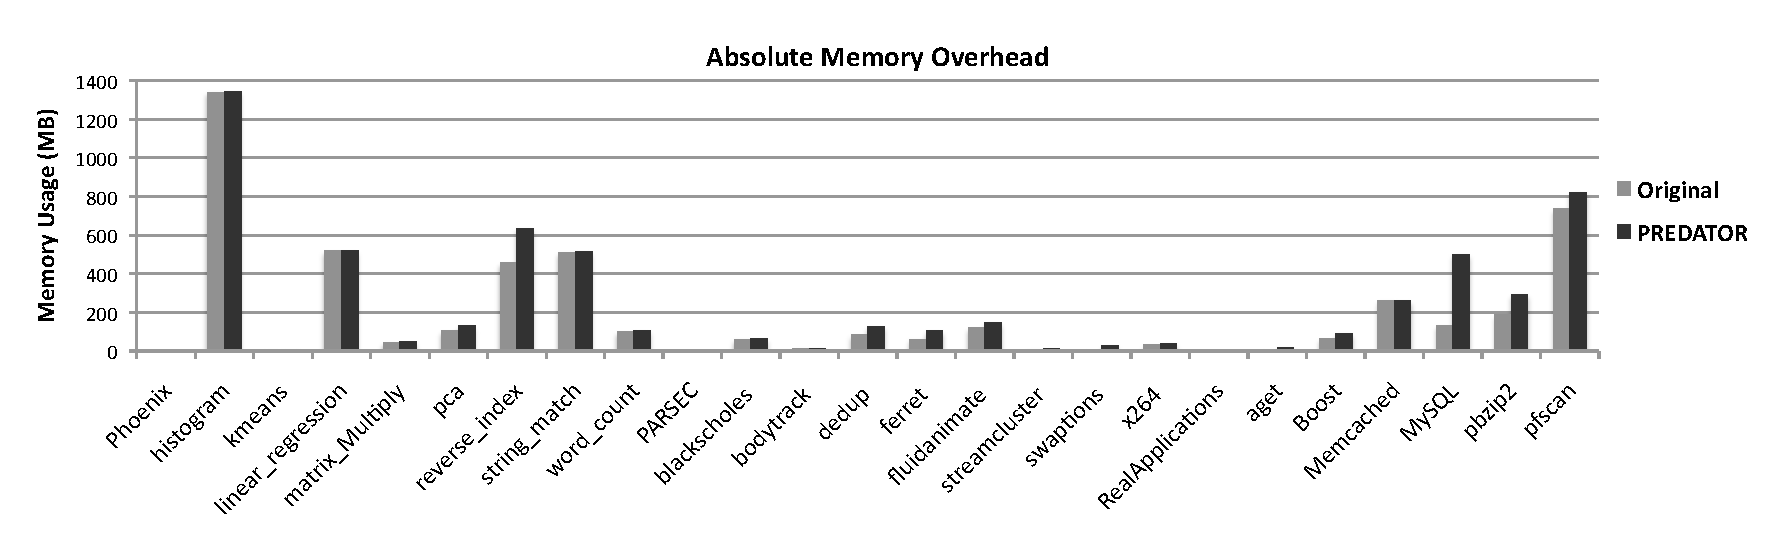
\includegraphics[width=6in]{predator/figure/absolutememory}
\caption{Absolute physical memory usage overhead with \Predator{}.}
\label{fig:absolutememusage}
\end{figure*}

\begin{figure*}[!t]
\centering
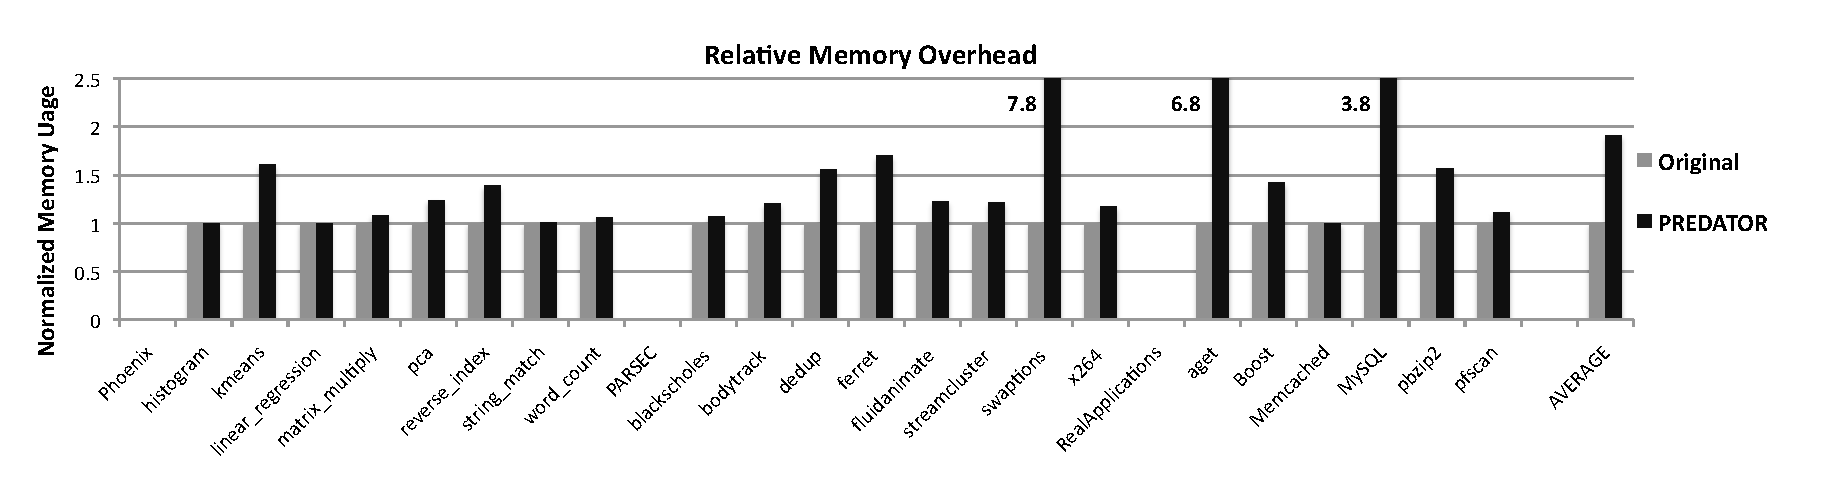
\includegraphics[width=6in]{predator/figure/memusage}
\caption{Relative physical memory usage overhead with \Predator{}.}
\label{fig:memusage}
\end{figure*}

\begin{figure}[!t]
\centering
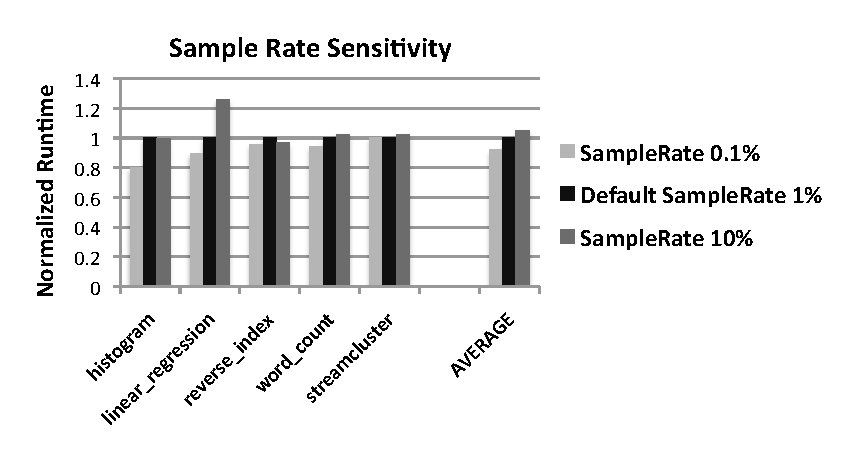
\includegraphics[width=6in]{predator/figure/sample}
%\includegraphics{fig/potential.pdf}
\caption{Sampling rate sensitivity (execution time).}
\label{fig:predatorsample}
\end{figure}


